\chapter{Импорт BPMN-схемы услуги}

Теперь перейдем к первому этапу проектирования нашего приложения
для услуги Совет да любовь - описания этого бизнес процесса в виде
графического представления в специальной нотации (BPMN).

В нашем случае, ознокомление с данной натацией было проведено в предудущей
лабораторной работе, и нам достаточно просто импортировать готовую схему
нашего процесса в проект (Рис. \ref{30-import}).

\myImage{Выбираем пункт <<Import process>>,
чтобы добавить готовую BPMN-диаграмму}{30-import}{30-import}

После чего мы можем в открывшемся окне \textit{Bizagi Modeler} подкорректоровать
при необходимости нашу схему (Рис \ref{30-description}). На схеме как раз
отображаются основные моменты проведения услуги: гражданин РФ, имеющий быть
честь предоставленный к награде <<Совет да любовь>>, может подать заявление
в многофункциональный центр (МФЦ), после чего в ходе некоторых проверок
(уточнение сведений о судимости в Информационном центре (ИЦ) и проверке соблюдения
прав детей заявителя) Министерство социальной политики заполняет наградной лист
и формулирует предложения о нагрождении, после чего передает все это в Правительство.

\begin{sidewaysfigure}
    \centering
    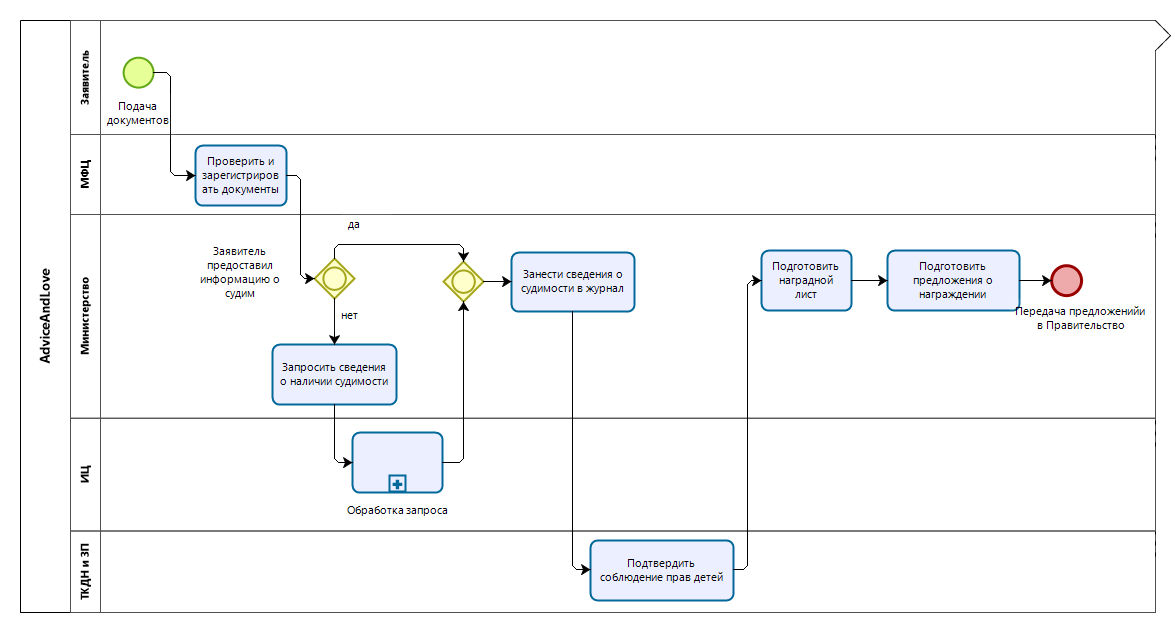
\includegraphics[width=\textwidth]{figures/30-BPMN}
    \caption{Улуга <<Совет да любовь>> в нотации BPMN}
    \label{30-description}
\end{sidewaysfigure}